\section{parte 04 – Desarrollo} 

\begin{enumerate}[1.]
	\item PROCEDIMIENTOS PARA LA CREACIÓN DE COPIAS:
\\
\\Primero se instaló la base de datos Oracle:
\\Oracle Database 11g Release 2 (11.2.0.1.0)
\\Standard Edition, Standard Edition One, and Enterprise Edition para Windows
\\
\\http://www.oracle.com/technetwork/database/enterprise-edition/downloads/112010-win64soft-094461.html
\\
\\Segundo se utilizó el programa sql developer para windows, esto fue para migrar la base de datos de mysql a oracle.
\\Si es que se requiera cambiar el puerto  oracle exec DBMS\_xdb.sethttpport(‘8082’);
\\
\\https://www.youtube.com/watch?v=-LJ\_370\_88g
\\
\\Las copias de seguridad o backups pueden ser físicas y lógicas:
\\
\\-Las físicas se realizan cuando se copian los ficheros que soportan la BD. Entre estos se encuentran los backups del SO, los backups en frío y los backups en caliente.
\\
\\
\textbf{ Backups del SO}         
\\           Este tipo de backup implica parar la BD en modo normal y esto la hace inaccesible el sistema mientras se lleva a cabo.
\\
\\
\textbf{ Backups de la BD en Frio}         
\\          Los backups en frio implican parar la BD en modo normal y copiar todos los ficheros sobre los que se asienta. Antes de parar la BD hay que parar también todas las aplicaciones que estén trabajando con la BD. Una vez realizada la copia de los ficheros, la BD se puede volver a arrancar.
\\
\\
\textbf{Backups de la BD en Caliente}            
\\          El backup en caliente se realiza mientras la BD está abierta y funcionando en modo ARCHIVELOG. Habrá que tener cuidado de realizarlo cuando la carga de la BD sea pequeña. Este tipo de backup consiste en copiar todos los ficheros correspondientes a un tablespace determinado, los ficheros redo log archivados y los ficheros de control.
\\

	\textbf{Backups Lógicos con Export/Import}  
	\\Estas utilidades permiten al DBA hacer copias de determinados objetos de la BD, así como restaurarlos o moverlos de una BD a otra. Estas herramientas utilizan comandos del SQL para obtener el contenido de los objetos.\\
	\\
	\\NOTA: Una vez que se ha planeado una estrategia de backup y se ha probado, conviene automatizarla para facilitar así su cumplimiento.

	\item BACKUPS  DESDE  ENTERPRISE  MANAGER:
	
\begin{center}
	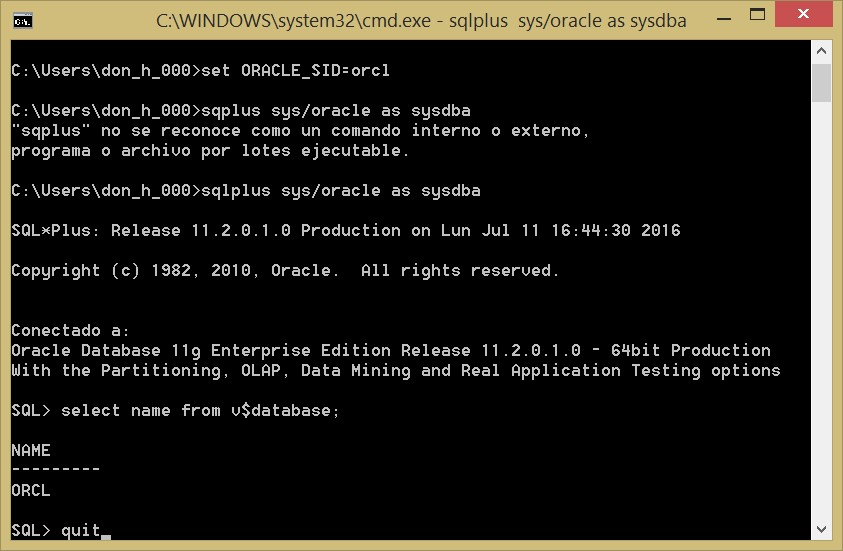
\includegraphics[width=15cm]{./Imagenes/img-4-2-1}  
	\end{center}
	Una  vez  logueados  en  EM,  iremos  al  apartado  “Disponibilidad”  y  apuntaremos  a “Planificar  Copia de Seguridad”.
	\begin{center}
	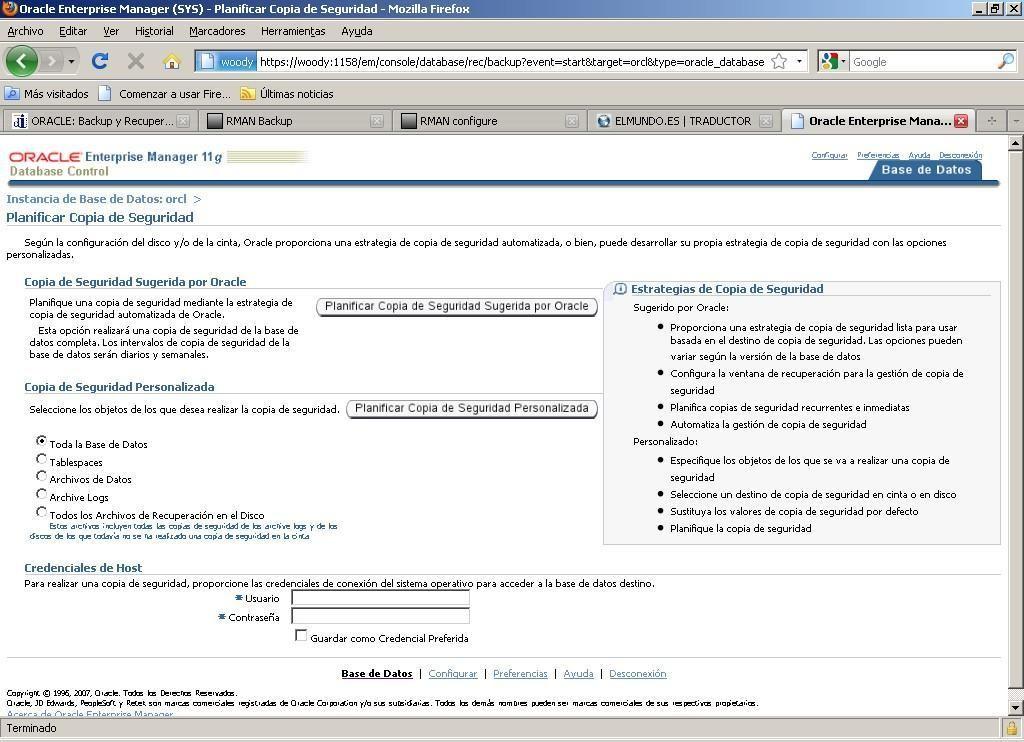
\includegraphics[width=15cm]{./Imagenes/img-4-2-2}  
	\end{center}
	Figura 3. Como vemos nos da 2 opciones a elegir. En este documento analizaremos la opción personalizada con toda la base de datos.
  	\\ Deberemos conectarnos con los credenciales de host para realizar esta tarea.
	\begin{center}
	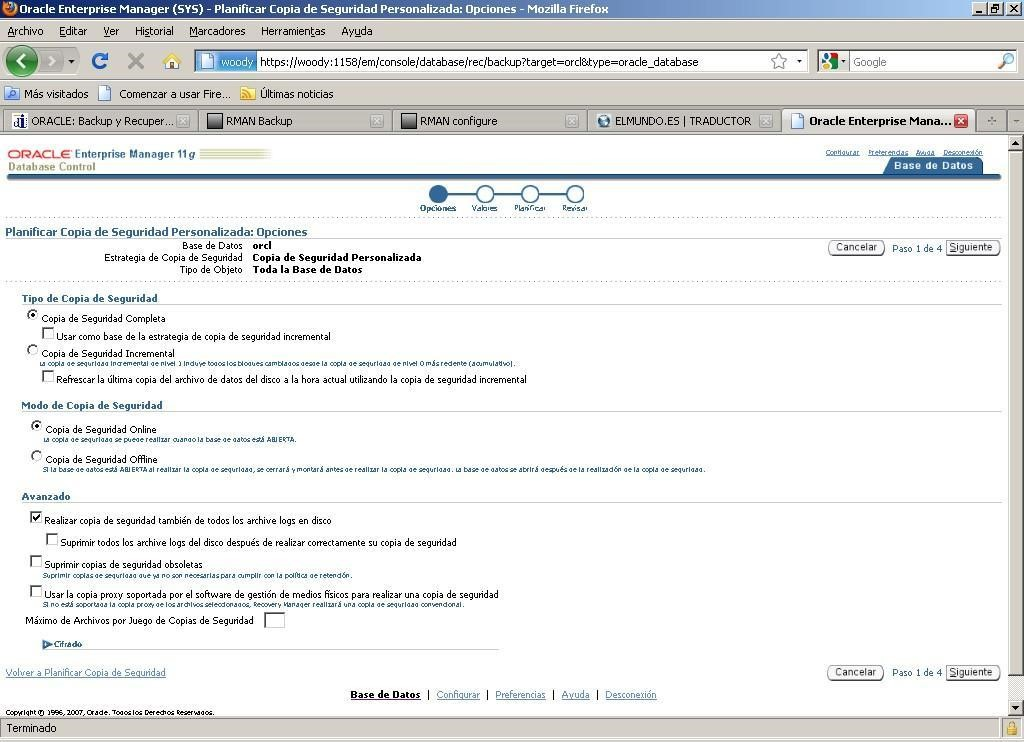
\includegraphics[width=15cm]{./Imagenes/img-4-2-3}  
	\end{center}
	Figura 4. Como  es  la  primera  copia  que  realizamos  deberíamos  elegir  “Copia  de  Seguridad Completa”
	\\Para el modo de copia elegiremos si deseamos hacer la copia con la base de datos abierta o cerrada. En las opciones avanzadas tan sólo añadiremos que realice copia también de los archive logs.
	\begin{center}
	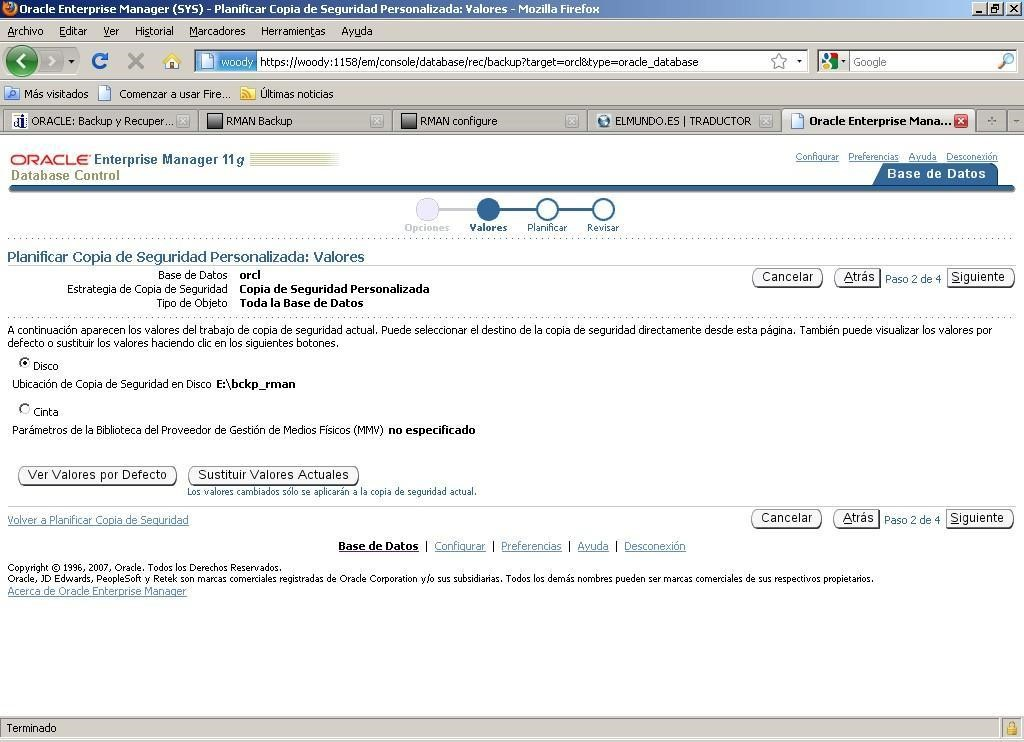
\includegraphics[width=15cm]{./Imagenes/img-4-2-4}  
	\end{center}
	Figura 5. En este paso elegiremos el destino de la copia. Como no dispongo de dispositivo de cintas pasó a continuar explicando la opción “Disco”. (La ubicación que ha tomado para la opción “Disco” está asignada desde RMAN).
	\begin{center}
	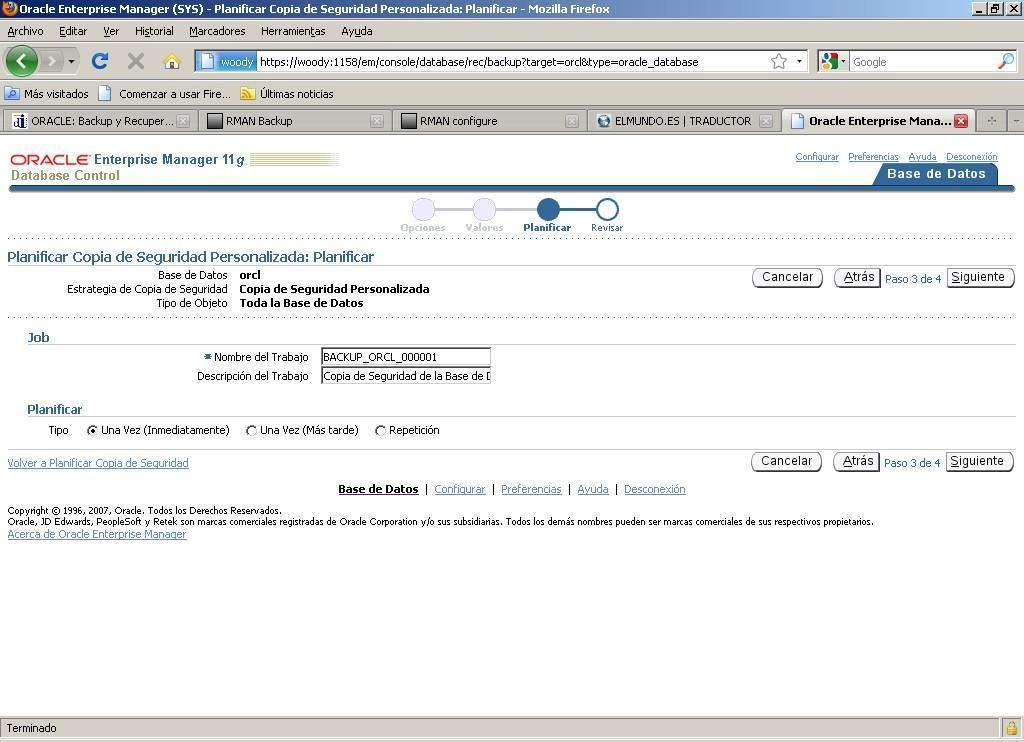
\includegraphics[width=15cm]{./Imagenes/img-4-2-5}  
	\end{center}
	Figura 6. Introducimos nombre si lo deseamos y la descripción, y lo planificamos para que se realice una vez y de forma inmediata.
	\begin{center}
	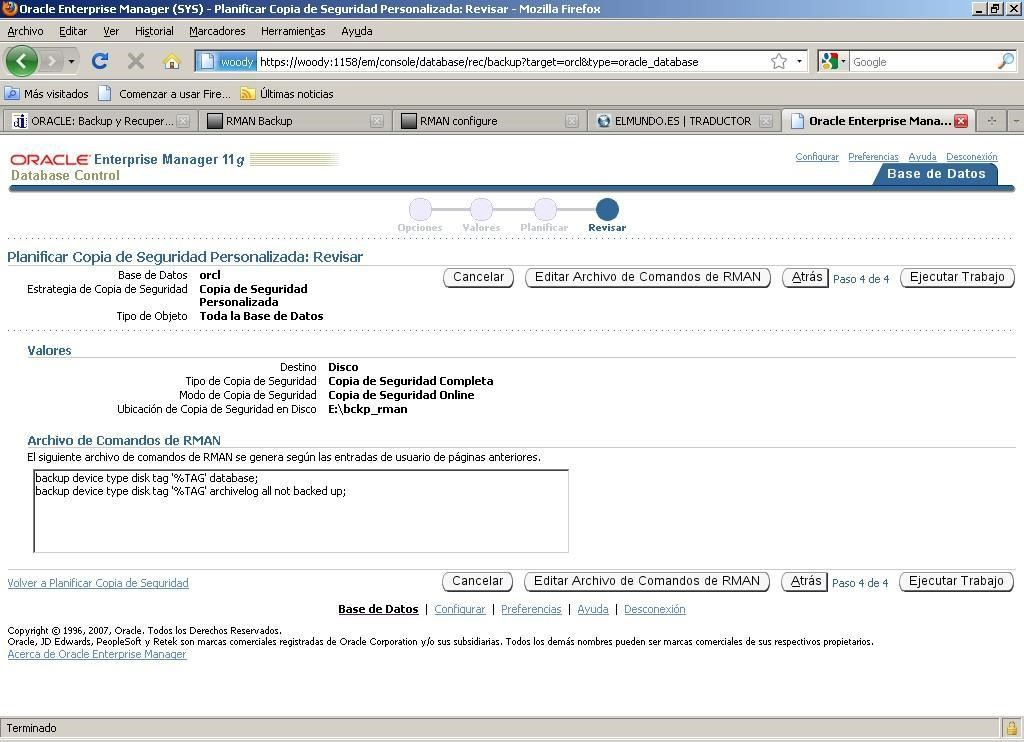
\includegraphics[width=15cm]{./Imagenes/img-4-2-6}  
	\end{center}
	Figura 7. Revisamos que todo esté correcto y ejecutamos el trabajo. Si todo ha ido bien debería aparecer esto:
	\begin{center}
	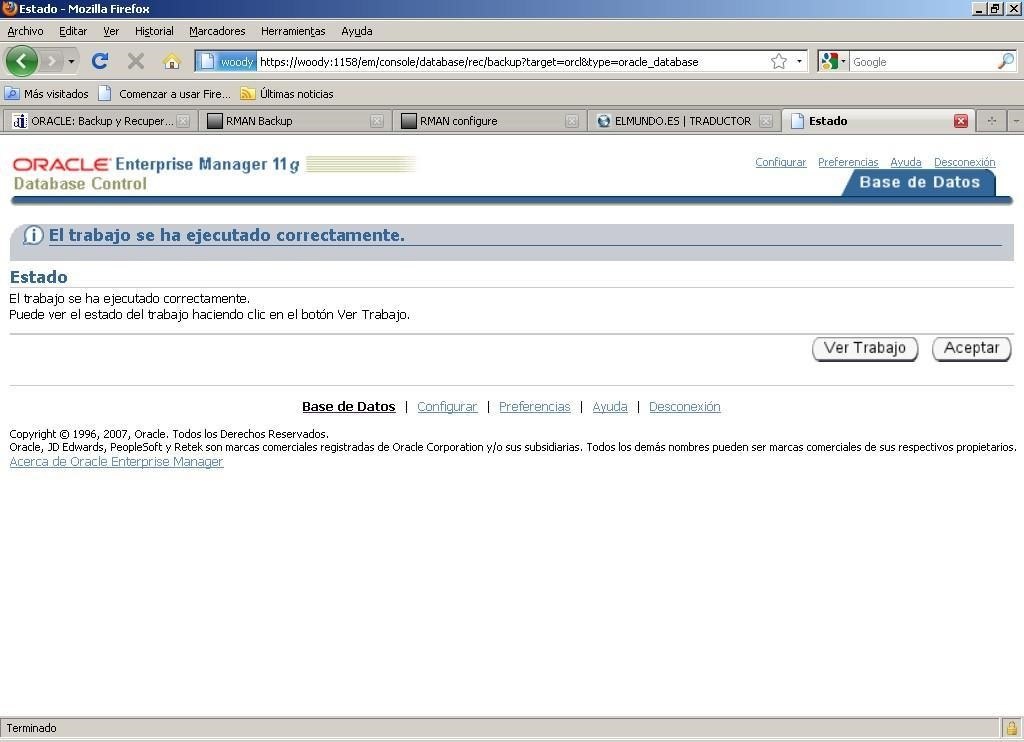
\includegraphics[width=15cm]{./Imagenes/img-4-2-7}  
	\end{center}



	\item RECUPERACIÓN  DESDE  ENTERPRISE  MANAGER
	\\\\Para realizar una recuperación desde EM, iremos a “Disponibilidad” y seleccionamos Realizar Recuperación
	\begin{center}
	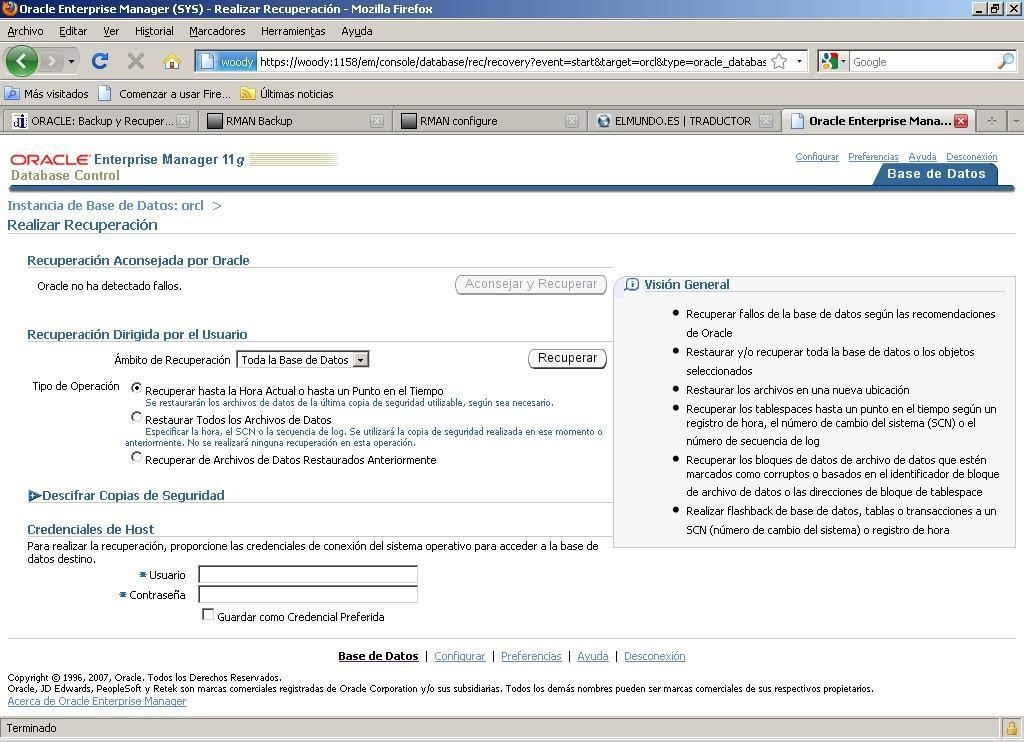
\includegraphics[width=15cm]{./Imagenes/recu_1}  
	\end{center}	
	En ámbitos de recuperación podemos seleccionar toda o parte de la base de datos para recuperar.
Para  el  ejemplo  hemos  borrado  el  datafile  USERS01.DBF(OFFLINE)  después  de realizar el backup y ahora vamos a intentar recuperarlo. Para ello usaremos la copia que acabamos de realizar. Iniciamos oracle en modo mount y arrancamos EM. Al no poder iniciar nos encontramos con esto una vez logueados.
	\begin{center}
	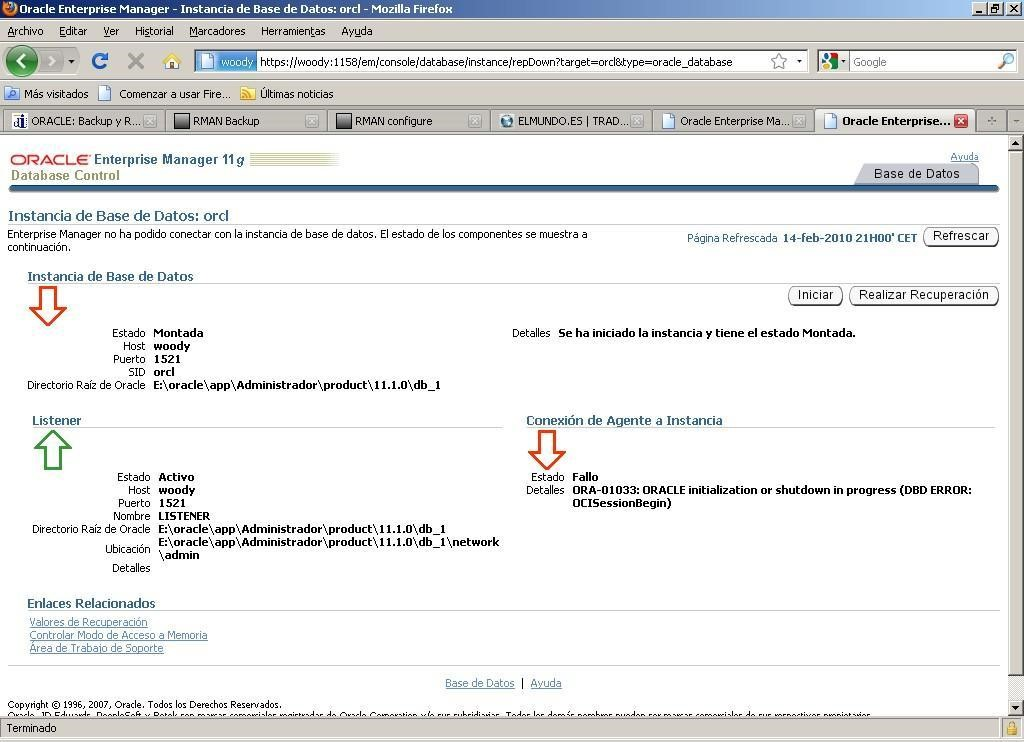
\includegraphics[width=15cm]{./Imagenes/recu_2}  
	\end{center}
	Pinchamos en Realizar Recuperación. Introducimos los credenciales de host. Continuar Nos conectamos como sysdba.
	\begin{center}
	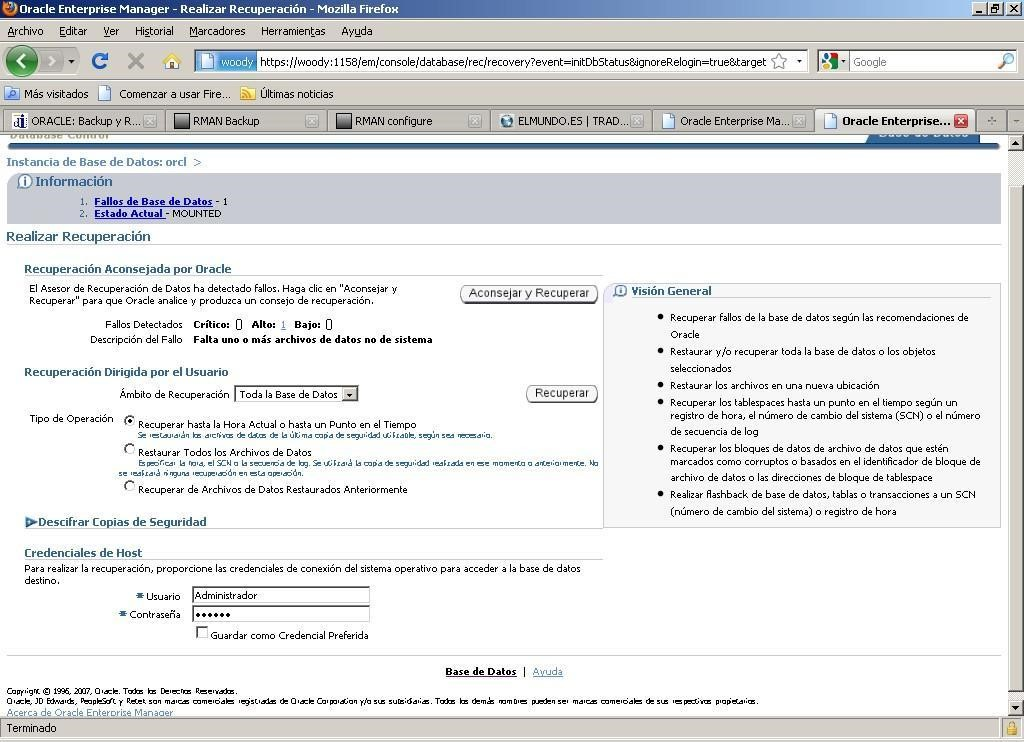
\includegraphics[width=15cm]{./Imagenes/recu_3}  
	\end{center}
	En el ámbito de recuperación elegimos Archivos de Datos y en el tipo de operación restaurar hasta hora actual. Pinchamos en recuperar.
	\begin{center}
	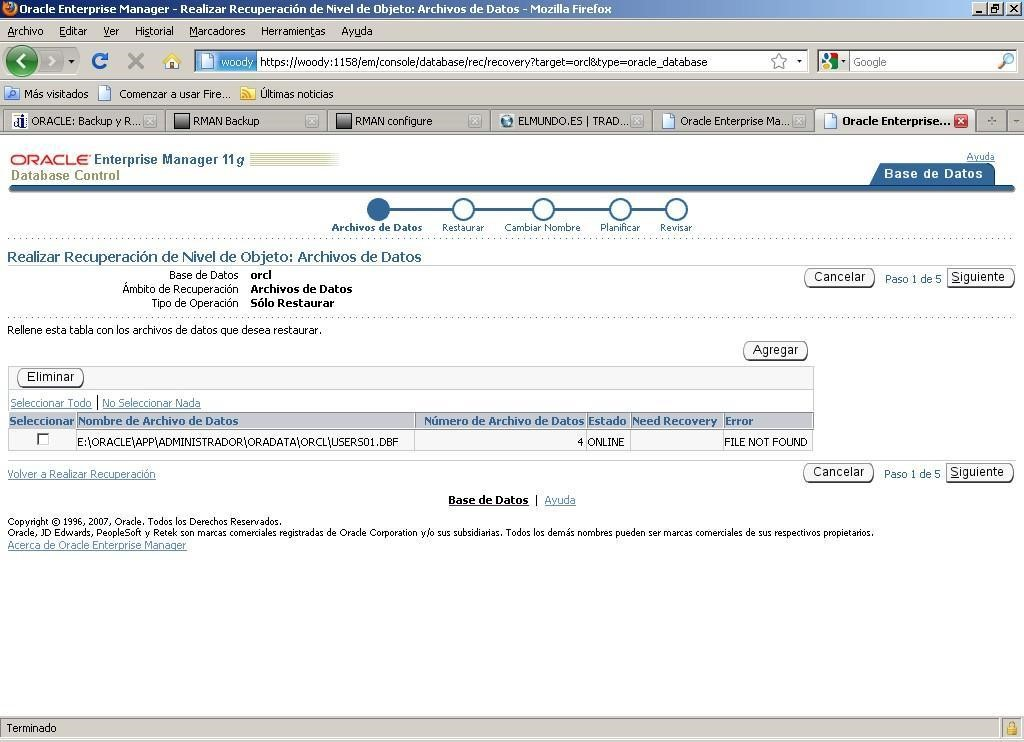
\includegraphics[width=15cm]{./Imagenes/recu_4}  
	\end{center}	
	Vemos  como  EM  localiza  la  ruta  en  conflicto  y  te  la  presenta  para  seleccionarla. Siguiente.
	\begin{center}
	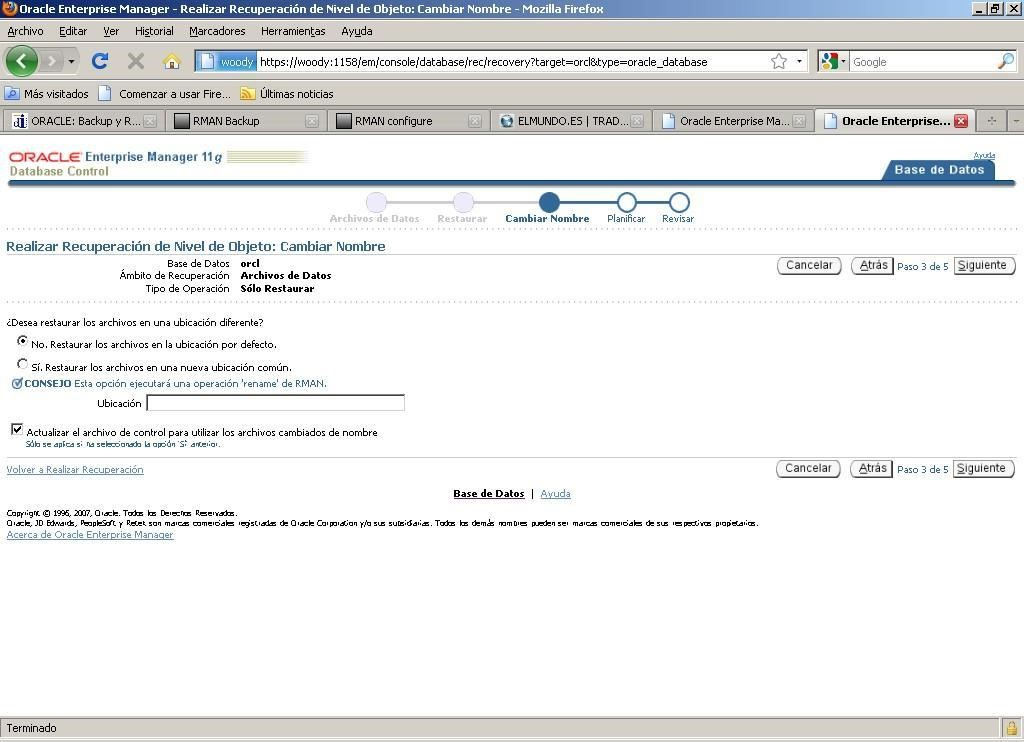
\includegraphics[width=15cm]{./Imagenes/recu_5}  
	\end{center}	
	También podemos definir el destino de la restauración. Para el ejemplo nos interesa que se ubiquen en el mismo directorio.
	\begin{center}
	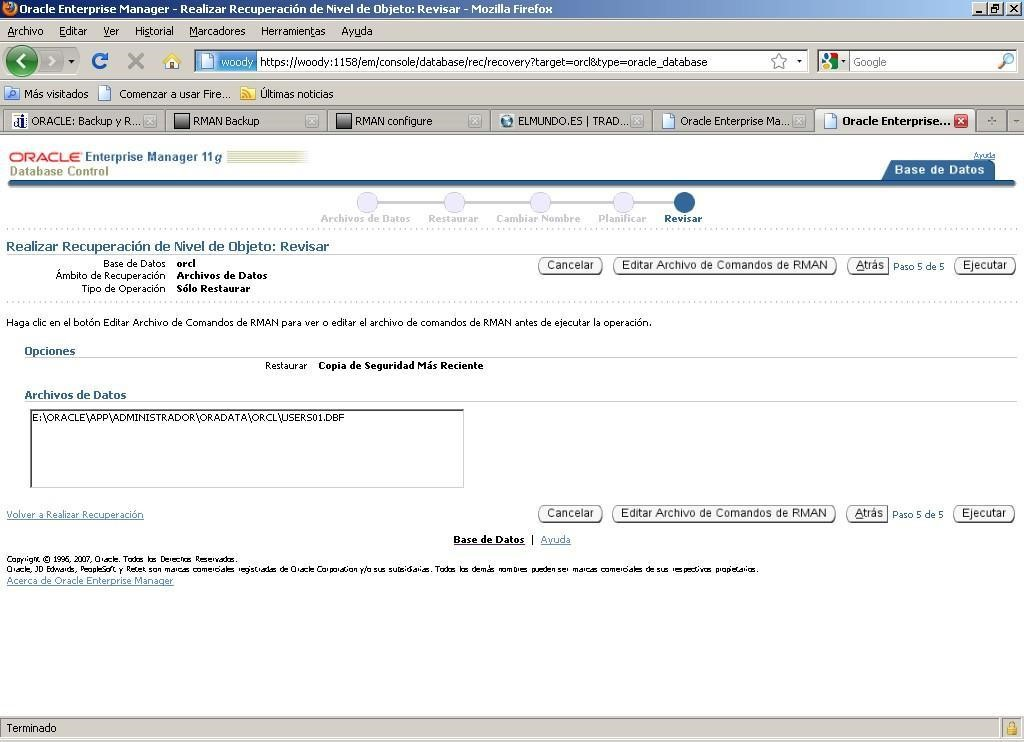
\includegraphics[width=15cm]{./Imagenes/recu_6}  
	\end{center}	
	Podemos revisar los parámetros RMAN para ver y comprender las acciones realizadas por debajo de EM. Una vez toda revisado procedemos a ejecutar.
	\\Esto lo que hará será tomar del backup el fichero y llevarlo al destino aplicando los cambios  hasta  el  momento  de  la  pérdida  permitiendo  así  el  inicio  normal  de  la  BD  con tablespace online.
	\\Una vez finalizado podemos pinchar en Abrir Base de Datos y esta se reiniciará y se abría automáticamente después de ver insertado nuestros credenciales.
	\begin{center}
	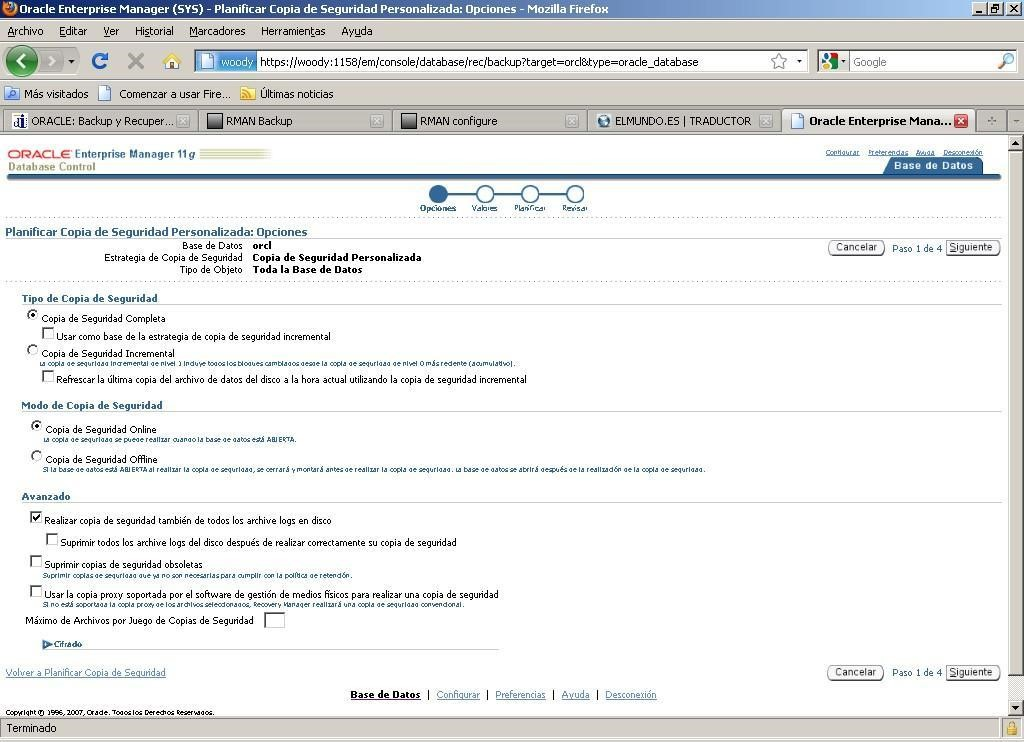
\includegraphics[width=15cm]{./Imagenes/eje1}
	\end{center}	
	Figura 5. En este paso elegiremos el destino de la copia. Como no dispongo de dispositivo de cintas paso a continuar explicando la opción Disco. La ubicacion que ha tomado para la opción  Disco  esta asignada desde RMAN
	\begin{center}
	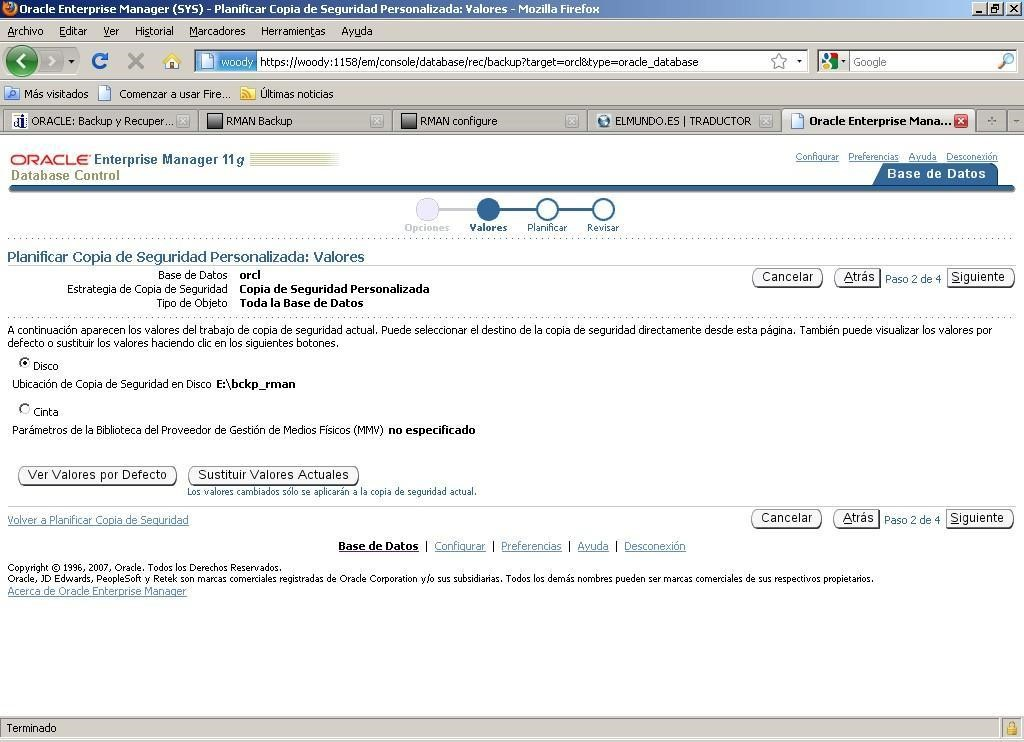
\includegraphics[width=15cm]{./Imagenes/eje2}
	\end{center}
	Figura 6. Introducimos nombre si lo deseamos y la descripcion, y lo planificamos para que se realice una vez y de forma inmediata
	\begin{center}
	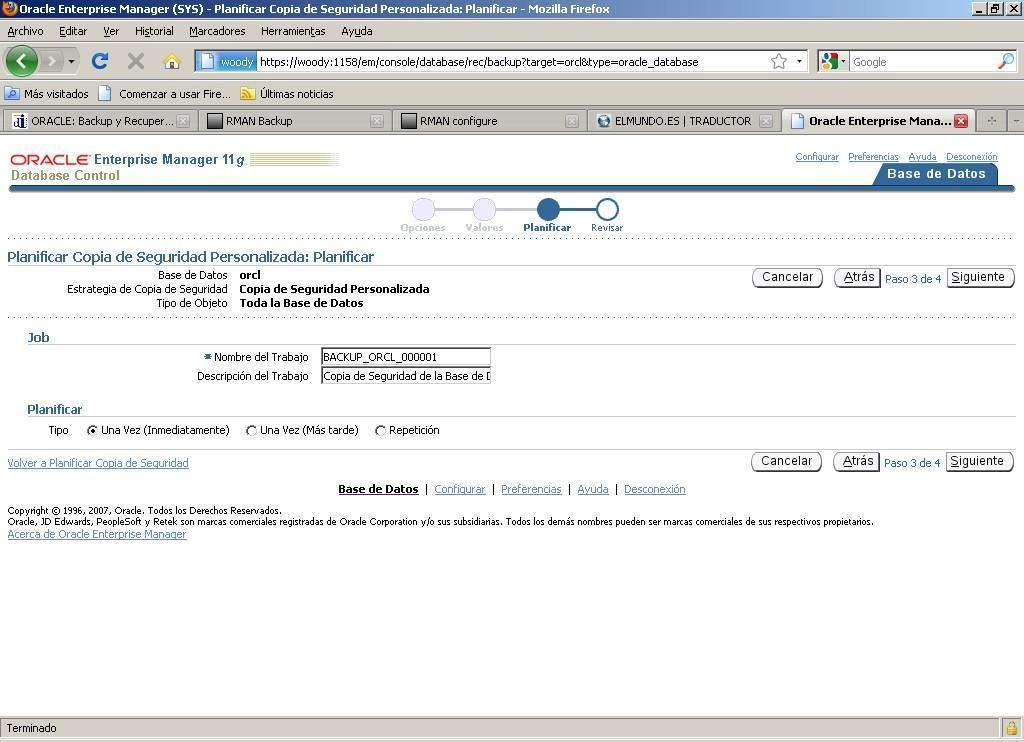
\includegraphics[width=15cm]{./Imagenes/eje3}
	\end{center}
	Figura 7. Revisamos que todo este correcto y ejecutamos el trabajo. Si todo ha ido bien deberia aparecer esto:
	\begin{center}
	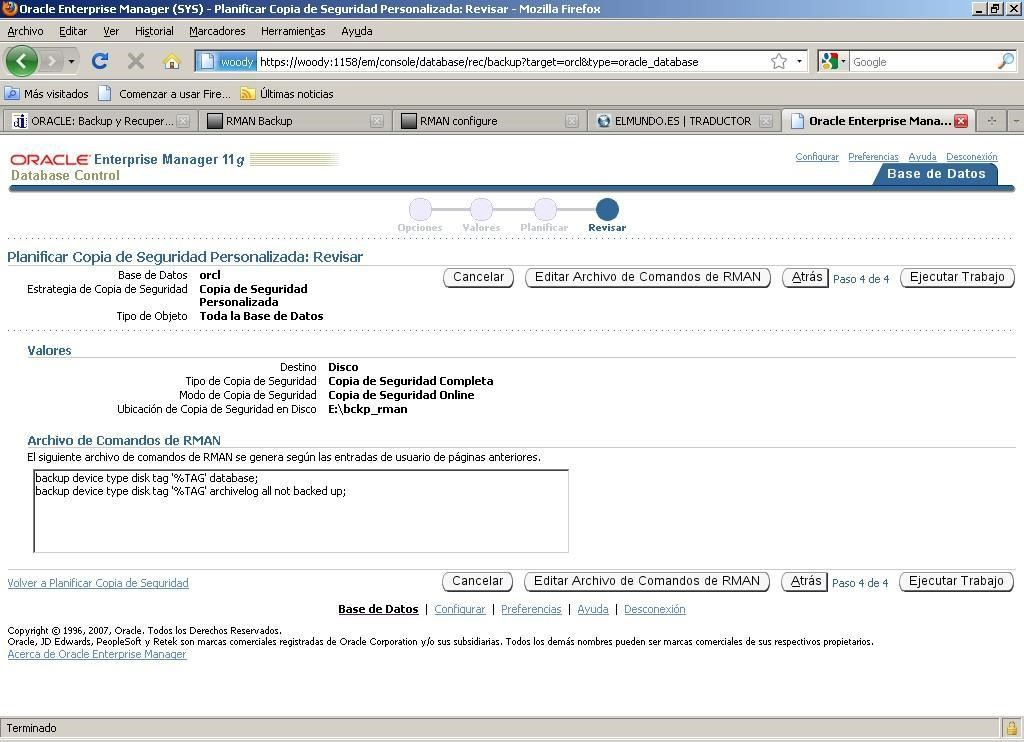
\includegraphics[width=15cm]{./Imagenes/eje4}
	\end{center}
	\\Recuperacion desde enterprise manager
	Para realizar una recuperación desde EM, iremos a Disponibilidad y seleccionamos
Realizar Recuperacion.
	\begin{center}
	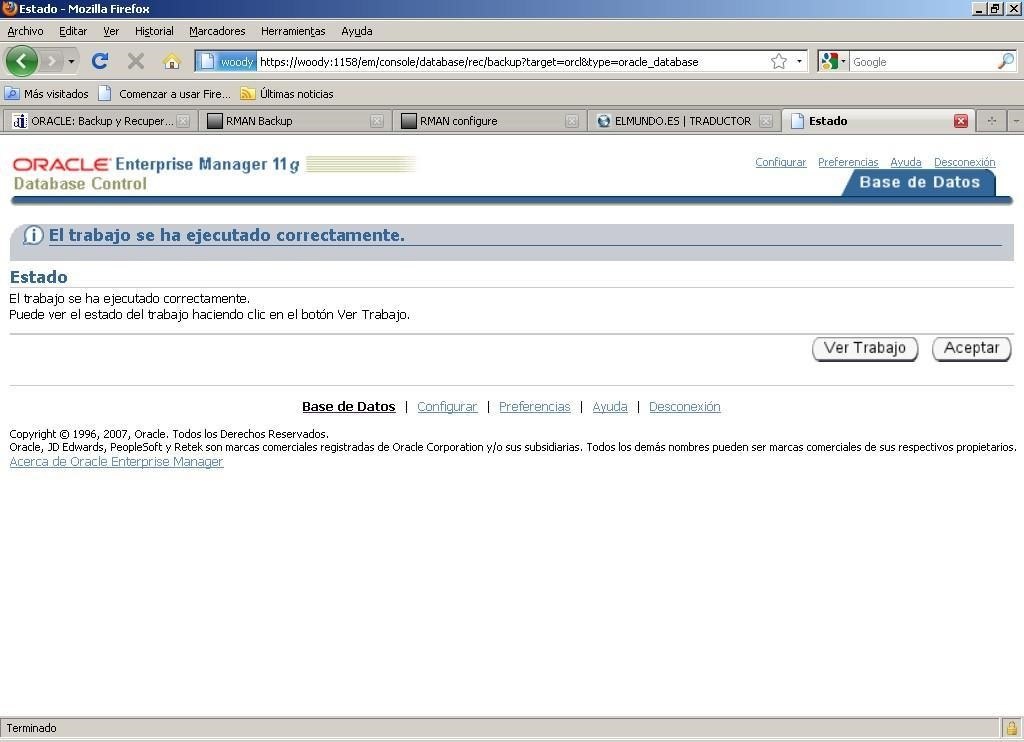
\includegraphics[width=15cm]{./Imagenes/eje5}
	\end{center}
Iniciamos oracle en modo mount y arrancamos EM
	\begin{center}
	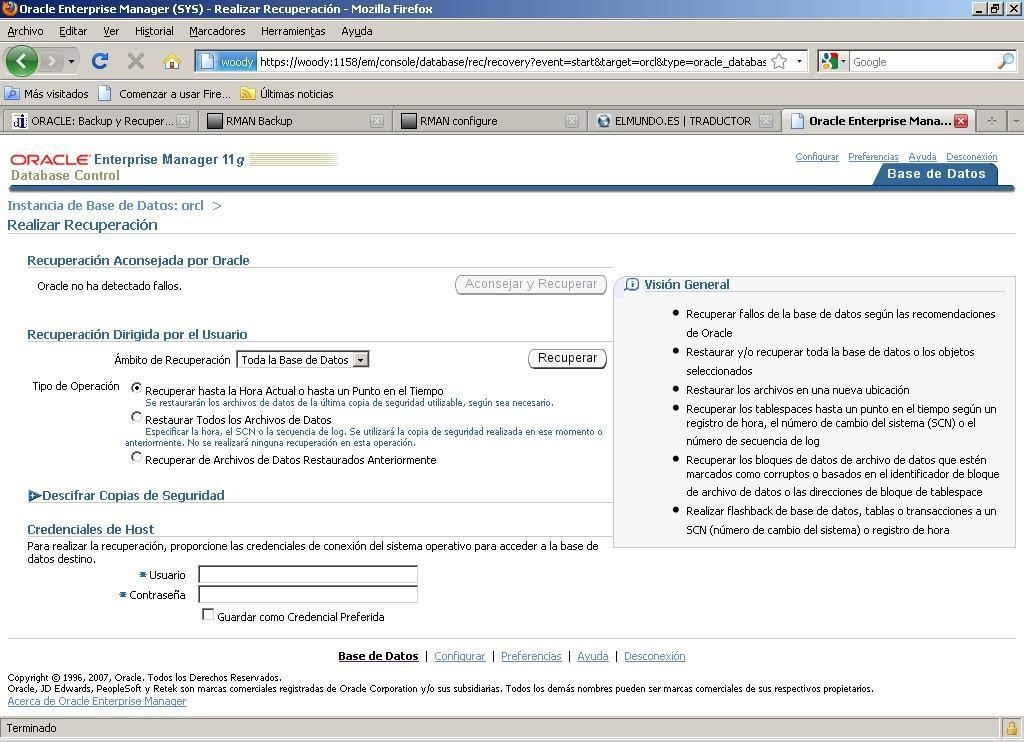
\includegraphics[width=15cm]{./Imagenes/eje6}
	\end{center}
	Pinchamos en Realizar Recuperacion. Introducimos los credenciales de host. Continuar Nos conectamos como sysdba.
	\begin{center}
	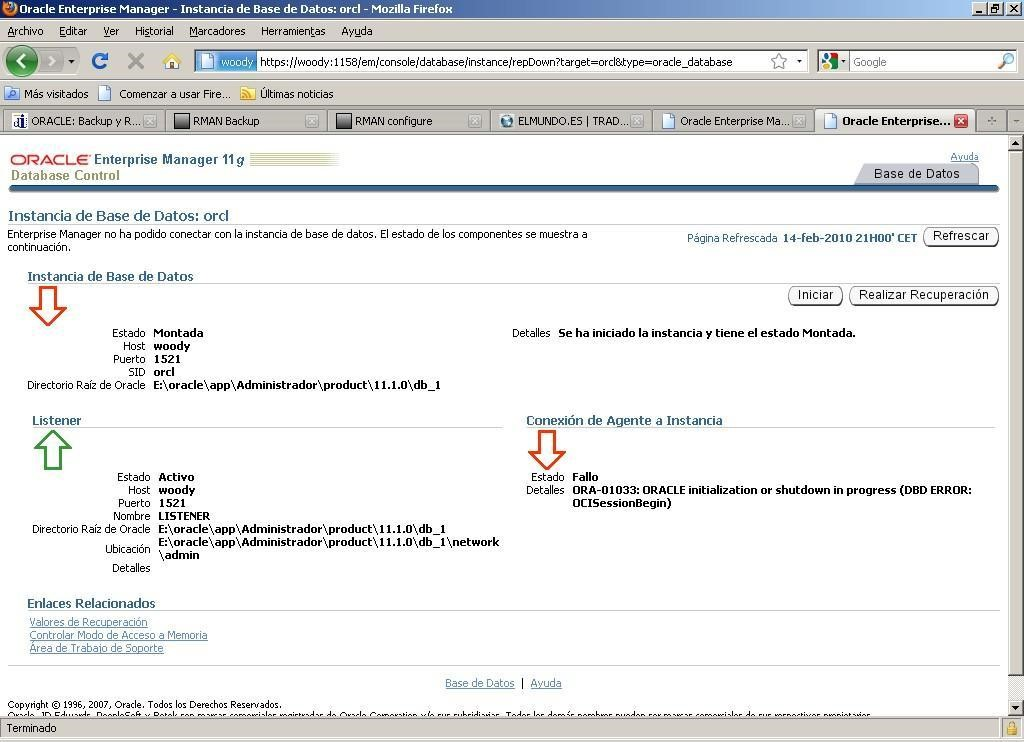
\includegraphics[width=15cm]{./Imagenes/eje7}
	\end{center}
	En el ámbito de recuperacion elegimos Archivos de Datos y en el tipo de operación restaurar hasta hora actual. Pinchamos en recuperar.
	\begin{center}
	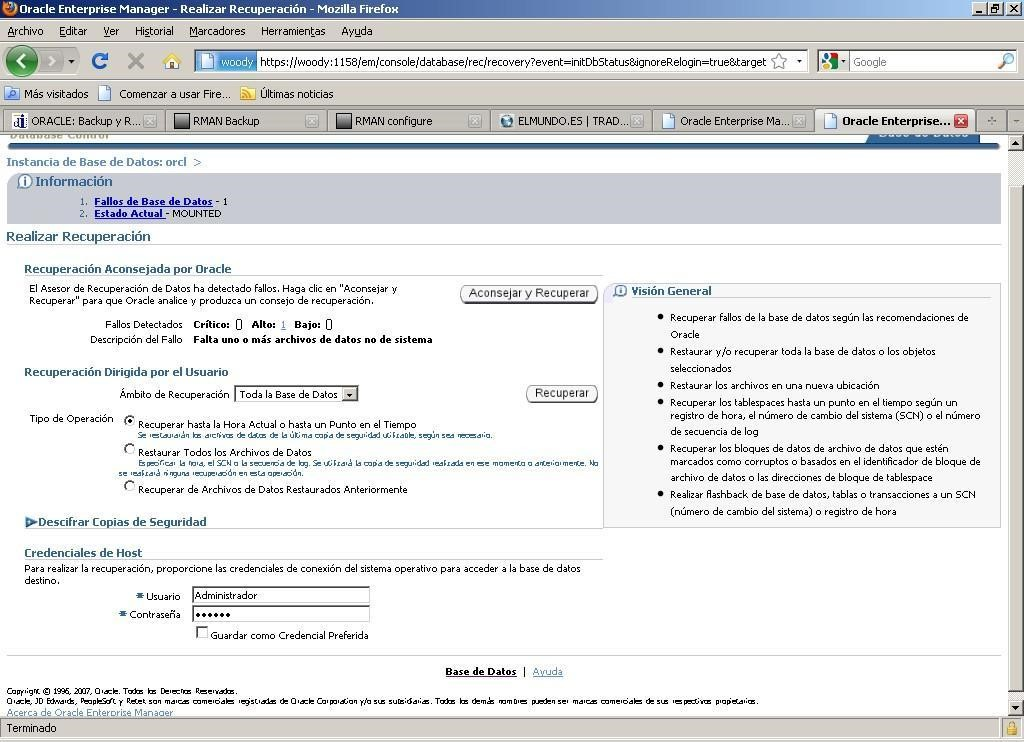
\includegraphics[width=15cm]{./Imagenes/eje8}
	\end{center}








\end{enumerate} 
